\documentclass[11pt]{article}
\usepackage{subfigure,wrapfig,booktabs,fancyhdr,amsmath,amsfonts,float}
\usepackage[pdftex]{graphicx}
\usepackage{bm,amssymb,amsmath,amsthm,wasysym,color,fullpage,setspace,multirow}
\usepackage{listings}
\lstset{language=Matlab}

\newcommand{\vb}{\boldsymbol}
\newcommand{\vbh}[1]{\hat{\boldsymbol{#1}}}
\newcommand{\vbb}[1]{\bar{\boldsymbol{#1}}}
\newcommand{\vbt}[1]{\tilde{\boldsymbol{#1}}}
\newcommand{\vbs}[1]{{\boldsymbol{#1}}^*}
\newcommand{\vbd}[1]{\dot{{\boldsymbol{#1}}}}
\newcommand{\vbdd}[1]{\ddot{{\boldsymbol{#1}}}}
\newcommand{\by}{\times}
\newcommand{\tr}{{\rm tr}}
\newcommand{\cpe}[1]{\left[{#1} \times \right]}
\newcommand{\sfrac}[2]{\textstyle \frac{#1}{#2}}
\newcommand{\ba}{\begin{array}}
\newcommand{\ea}{\end{array}}
\renewcommand{\earth}{\oplus}
\newcommand{\sinc}{{\rm \hspace{0.5mm} sinc}}
\newcommand{\tf}{\tilde{f}}
\newcommand{\tbox}[1]{\noindent \fbox{\parbox{\textwidth}{#1}}}
\DeclareMathAlphabet{\mathpzc}{OT1}{pzc}{m}{it}

% Weird thing I have to add to allow `rubber` to compile
\DeclareUnicodeCharacter{2212}{-}

\title{ASE 389P-7 \\ Exam 1}
\author{Alejandro Moreno}\date{October 4, 2022}

\begin{document}
%\onehalfspace
\maketitle

\section{Problem 1}

\subsection{Instruction}

Write a function in Matlab that simulates the train-horn-Doppler scenario
discussed in lecture. Assume that the train tracks are rectilinear.

Be sure to account for the nonzero time of flight $\delta t_{TOF}$ as discussed
in lecture. The effect of $\delta t_{TOF} > 0$ is that the stationary observer
will discern an $f_D$ at time $t_k$ that relates to the train’s line-of-sight
velocity at time $t_k − \delta t_{TOF}$. More precisely, the apparent frequency
of the train horn at the location of the observer at time $t_k$ is given by

\begin{equation}
	f_r(t_k) = \frac{f_c}{1 + \frac{v_{los}(t_k)}{v_s}}
\end{equation}

where $f_c$ is the nominal horn frequency, $v_{los}(t_k)$ is the line-of-sight
velocity at $t_k$, and $v_s$ is the speed of the signal in the medium. Note that
the line-of-sight geometry used to calculate $v_{los}(t_k)$  is between the
observer at time $t_k$ and the horn at time $t_k − \delta t_{TOF}$.

Download the audio file trainout.wav from Canvas. This file was created with the
following input argument values:

\begin{lstlisting}
  fh = 440;
  vTrain = 20;
  t0 = 0;
  x0 = 0;
  delt = 0.01;
  N = 1000;
  vs = 343;
\end{lstlisting}

Set up your simulator with these same values. Estimate the values of xObs and
dObs by adjusting them in your simulation until you get an apparent received
frequency profile that matches the one in the audio file.

\subsection{MATLAB code}

\lstinputlisting{simulateTrainDoppler.m}
\lstinputlisting{topSimulateTrainDoppler_temp.m}

\subsection{Result}

Analizing the given signal it's possible to manually tag the moment in which the
train passed in front of the receiver. Figure~\ref{fig:spectrogram_original}
shows how the power density is concentrated at higher frequency before 3.069 sec
and drops rapidly after that. This indicates the exact moment at which the train
passed infront of the receiver.

\begin{figure}[H]
	\centering
	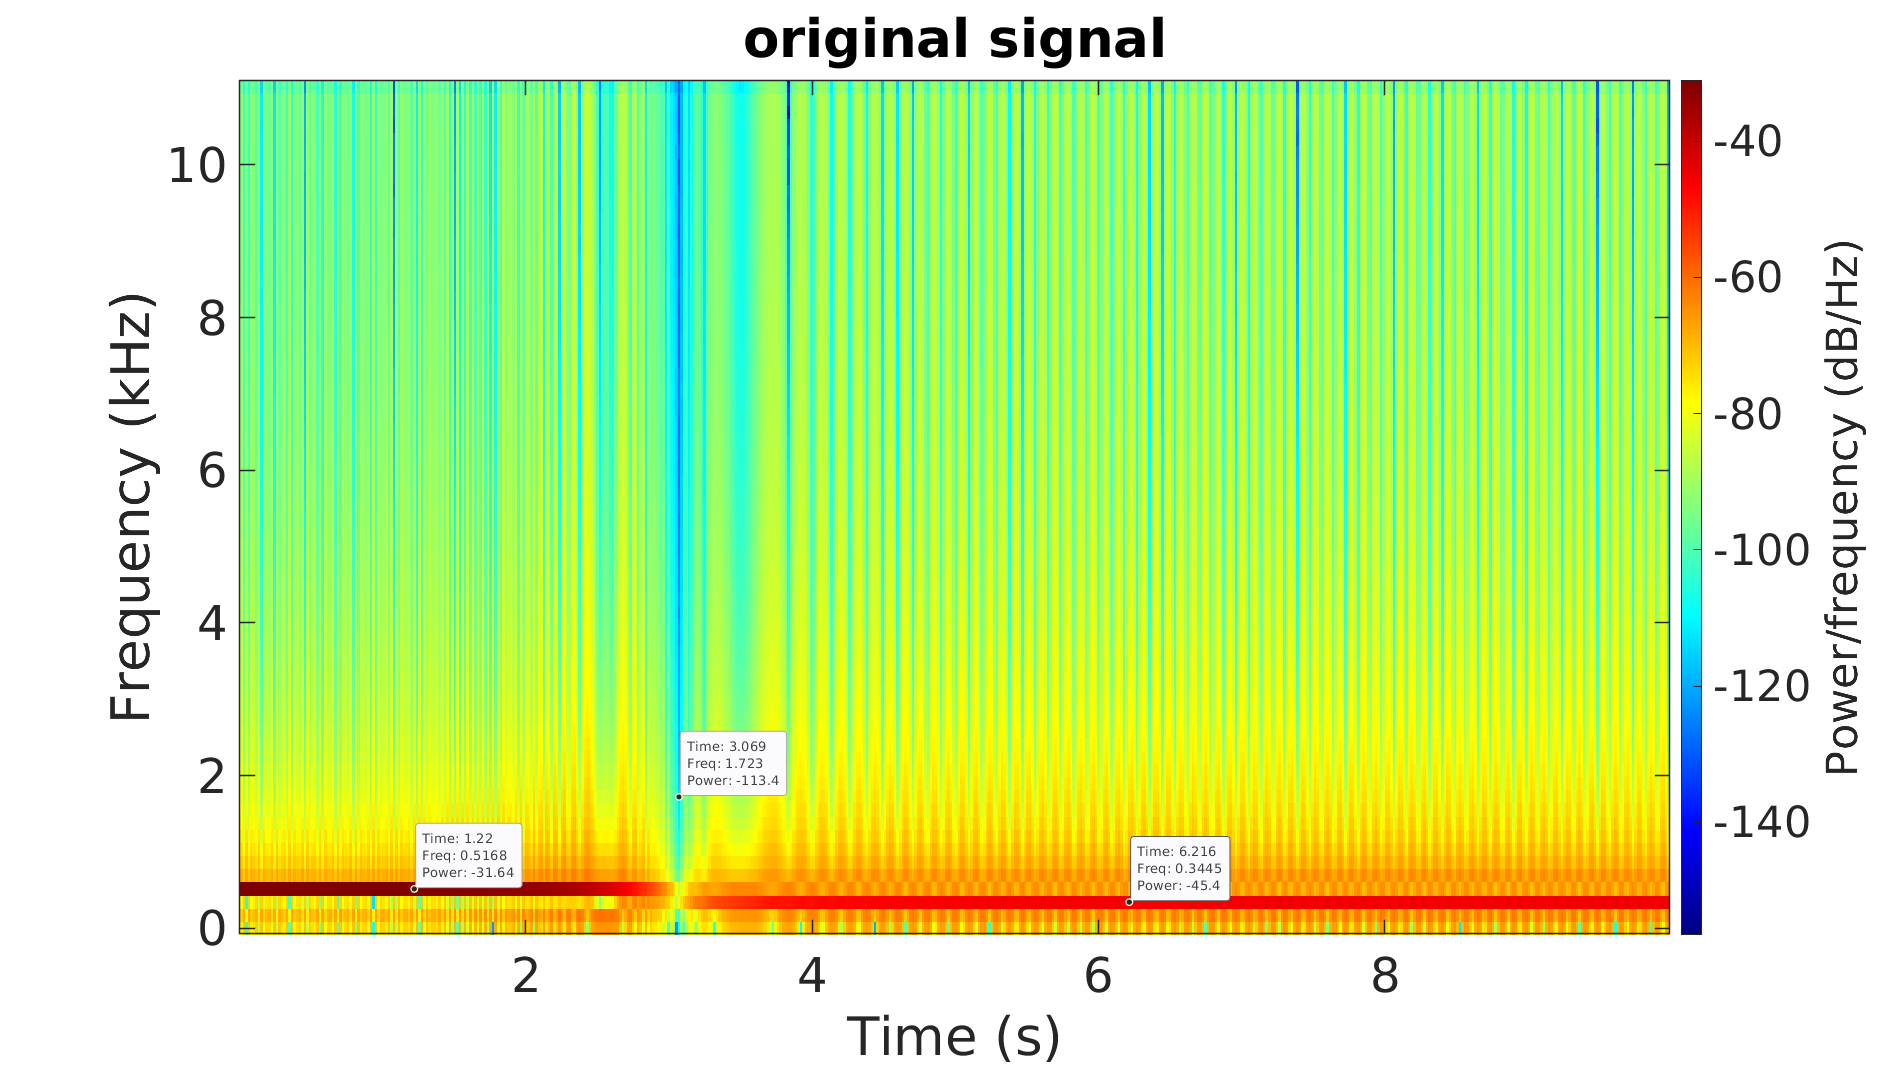
\includegraphics[width=0.9\textwidth]{figs/ex1_spectrogram_orig.png}
	\caption{Spectrogram of the given signal.}
	\label{fig:spectrogram_original}
\end{figure}

This, approach lead to $xObs = 56.8$ and $dObs = 10$.




\section{Problem 2}

\subsection{Instruction}

Show that the group velocity vg and the phase index of refraction np are related
by $v_g = c \eta_p$ for small group and phase velocity departures from the speed
of light $c$.

\subsection{Solution}



\section{Problem 3}

\subsection{Instruction}

In lecture we considered an analog signal $x_a (t)$ sampled by impulses:

\begin{equation}
	x_\delta (t) = \sum_{n=-\infty}^{\infty} x_a(nT) \delta(t-nT)
	\label{eq:ex3_analog_signal}
\end{equation}

We showed that the Fourier transform of the impulse-sampled signal $x_\delta (t)$
is related to $X_a (f)$, the Fourier transform of $x_a (t)$, by

\begin{equation}
	X_\delta (f) = \frac{1}{T} \sum_{n=-\infty}^{\infty} X_a(f- \frac{n}{T})
	\label{eq:ex3_FT_sampled_signal}
\end{equation}

We can derive a similar relationship between $X_a (f)$ and the Fourier transform
of the discrete-time signal

\begin{equation}
	x(n) = x_a (nT), − \infty < n < \infty
\end{equation}

To make this easier, we’ll define the frequency variable
$\tilde{f} = f T = \frac{f}{f_s}$. This variable, which has units of cycles per
sample and is often called the normalized frequency, is used as the frequency
variable for discrete-time signals. For example, a discrete-time sinusoid can be
represented as $2x(n) = cos(2\pi \tilde{f}n)$. For discrete-time signals, only
frequencies in the range $− 1/2 \le \tilde{f} \le 1/2$ are unique;
all frequencies $|\tilde{f}| > 1/2$ are aliases.

The Fourier transform of a discrete-time signal $x(n)$ is defined by

\begin{equation}
	X(\tilde{f}) = \sum_{n=-\infty}^{\infty} x(n) \exp{(-j 2 \pi \tilde{f} n)}
	\label{eq:ex3_DFT}
\end{equation}

and the inverse transform is defined by

\begin{equation}
	x(n) = \int_{-1/2}^{1/2} X(\tilde{f}) \exp{(j 2 \pi \tilde{f} n)} d\tilde{f}
	\label{eq:ex3_IDFT}
\end{equation}

Derive the relationship between $X(\tilde{f})$ and $X_a (f)$.

\textbf{Hint:} This is a standard relationship whose derivation can be found in
many texts that treat digital signal processing. You’re free to use such a text
as a guide or you may perform the derivation yourself following these steps:

\begin{itemize}
	\item Express $x(n) = x_a (nT)$ in terms of $X_a (f)$.
	\item Equate this expression with the inverse transform definition given above.
	\item Express the integral that goes from $−\infty to \infty$ as an infinite
	      sum of integrals of width $f_s$.
	\item Make a change of variable $f = \tilde{f}  fs$ in this infinite sum of
	      integrals expression to eliminate $f$ in favor of $\tilde{f}$.
	\item Make some deductions to arrive at the desired relationship between
	      $X(\tilde{f})$ and $X_a (f = \tilde{f}·fs )$.
\end{itemize}

\subsection{Solution}

It is possible to consider equation~\ref{eq:ex3_analog_signal} to calculate the
Fourier Transform of $x_\delta(t)$.

\begin{equation}
	X_\delta (f) = \frac{1}{T} \sum_{n=-\infty}^{\infty} X_a(f- \frac{n}{T})
	= \sum_{n=-\infty}^{\infty} x_a(nT) \exp{(-j 2 \pi f n T)}
\end{equation}

Then, it is possible to see that formula for $X_\delta (f)$ can be equated to
\ref{eq:ex3_DFT} as follows

\begin{equation}
	X_\delta (f) = \sum_{n=-\infty}^{\infty} x_a(nT) \exp{(-j 2 \pi f n T)}
	= \sum_{n=-\infty}^{\infty} x(n) \exp{(-j 2 \pi \tilde{f} n)}
	= X(\tilde{f})
\end{equation}

This leads to the following relationship

\begin{equation}
	X(\tilde{f}) = X_\delta (\frac{\tilde{f}}{T})
\end{equation}

Now, using equation~\ref{eq:ex3_FT_sampled_signal} it is possible to reach

\begin{equation}
	X(\tilde{f}) = \frac{1}{T} \sum_{n=-\infty}^{\infty} X_a(\frac{\tilde{f}- n}{T})
\end{equation}


%\bibliographystyle{ieeetr}
%\bibliography{./pangea}  
\end{document}
